% pet_pbt_talk.tex — CRYSP in-room PET for proton-therapy range verification.
% Talk for a medical-institute audience (physicians, potential collaborators).
% Figures in latex/figs/. Compile: pdflatex pet_pbt_talk.tex (x2 for the outline).
\documentclass[aspectratio=169,11pt]{beamer}

\usepackage[T1]{fontenc}
\usepackage[utf8]{inputenc}
\usepackage{helvet}
\usepackage{graphicx}
\usepackage{booktabs}
\usepackage{amsmath}
\usepackage{tikz}
\usepackage{eurosym}
\usetikzlibrary{shapes.geometric, arrows.meta, positioning, backgrounds}

\graphicspath{{figs/}}

% ---- clean custom look (no external theme needed) --------------------------
\usetheme{default}
\setbeamertemplate{navigation symbols}{}
\definecolor{crBlue}{RGB}{22,88,138}
\definecolor{crRed}{RGB}{200,74,40}
\definecolor{crGrey}{RGB}{90,95,100}
\setbeamercolor{title}{fg=crBlue}
\setbeamercolor{frametitle}{fg=crBlue}
\setbeamercolor{structure}{fg=crBlue}
\setbeamercolor{normal text}{fg=black}
\setbeamerfont{frametitle}{series=\bfseries, size=\large}
\setbeamerfont{title}{series=\bfseries}
\setbeamertemplate{itemize item}{\color{crRed}\textbullet}
\setbeamertemplate{itemize subitem}{\color{crGrey}--}
\setbeamertemplate{frametitle}{%
  \vspace{3mm}\hspace{2mm}%
  {\usebeamerfont{frametitle}\usebeamercolor[fg]{frametitle}\insertframetitle}\par
  \hspace{2mm}{\color{crBlue}\rule{0.965\paperwidth}{1.1pt}}\vspace{-1mm}}
\setbeamertemplate{footline}{%
  \hbox{}\hfill{\color{crGrey}\scriptsize\insertframenumber\,/\,\inserttotalframenumber}%
  \hspace{3mm}\vspace{2mm}}

\newcommand{\OT}{\textsuperscript{15}O}
\newcommand{\CE}{\textsuperscript{11}C}
\newcommand{\hi}[1]{\textcolor{crRed}{#1}}

\title[CRYSP in-room PET for PBT]{A High-Sensitivity In-Room \textbf{CRYSP} Scanner\\
  for Distal-Edge Verification in Proton Therapy}
\author{J.J.\ G\'omez-Cadenas, F.\ L\'opez-Guejo and R.\ Soleti}
\date{\small BioGipuzkoa \\ \today}

\begin{document}

{\setbeamertemplate{footline}{}
\begin{frame}[plain]
  \titlepage
\end{frame}}

% ===========================================================================
\section{PET for proton therapy}

% Definition: https://www.cancer.gov/about-cancer/treatment/types/radiation-therapy/external-beam
% Image: https://commons.wikimedia.org/wiki/File:BraggPeak-en.svg
% CC0; vectorization by D. Ilyin, based on BraggPeak.png by Dr A. A. Miller.
\begin{frame}{What is proton therapy?}
  \small
  \begin{columns}[T]
    \begin{column}{0.52\textwidth}
      \begin{itemize}
        \item A form of \hi{external-beam radiotherapy} that uses
          accelerated protons to destroy tumour cells.
        \item Protons are \hi{positively charged particles}:
          their energy determines how deep they travel in tissue.
        \item Their dose peaks near the end of their range
          (the \hi{Bragg peak}), then falls sharply.
        \item Combining different proton energies covers the tumour
          volume, while \hi{reducing dose beyond it} compared with X-rays.
      \end{itemize}
    \end{column}
    \begin{column}{0.48\textwidth}
      \centering
      
\includegraphics[width=\linewidth]{proton_therapy_bragg.png}\\[1mm]
      {\scriptsize\color{crGrey} Schematic depth--dose profiles: a single
       proton energy, a spread-out peak and an X-ray beam.}\\[2mm]
      {\tiny\color{crGrey}
       \href{https://commons.wikimedia.org/wiki/File:BraggPeak-en.svg}
       {Image: D. Ilyin / A. A. Miller, Wikimedia Commons (CC0).}\\
       \href{https://www.cancer.gov/about-cancer/treatment/types/radiation-therapy/external-beam}
       {Reference: National Cancer Institute, External Beam Radiation Therapy.}}
    \end{column}
  \end{columns}
\end{frame}

% Incidence estimates: NCI Childhood Brain and Spinal Cord Tumors Summary Index
% (CBTRUS 2006--2010), and NCI Childhood Ependymoma.
\begin{frame}{Example: Brain tumors}
  \small
  \begin{columns}[T]
    \begin{column}{0.58\textwidth}
      \begin{itemize}
        \item Brain tumours are the \hi{most common solid tumours in children}:
          about \hi{300 diagnoses/year in Spain}, and also common in adults ($\sim$ 4500 cases per year).
        \item One example of brain tumour (ependymomas) often arise around the fourth
          ventricle, close to critical structures such as the
          \hi{cerebellum and brainstem}.
        \item The goal and crucial challenge of radiotherapy is to
          \hi{fully cover the tumour} with the prescribed dose while
          \hi{sparing these nearby structures}.
      \end{itemize}
    \end{column}
    \begin{column}{0.42\textwidth}
      \centering
      
\includegraphics[width=\linewidth,height=0.42\textheight,keepaspectratio]{ependymoma_mri.png}\\
      {\scriptsize\color{crGrey} Fourth-ventricle ependymoma (MRI).}\\[3mm]
      {\tiny\color{crGrey} Sources: National Cancer Institute\\
       \href{https://www.cancer.gov/types/brain/hp/child-brain-treatment-pdq}
       {Childhood Brain and Spinal Cord Tumors (PDQ)};\\
       \href{https://www.cancer.gov/types/brain/patient/childhood-ependymoma}
       {Childhood Ependymoma}.}
    \end{column}
  \end{columns}
\end{frame}

\begin{frame}{Proton therapy: a sharp tool that must be aimed precisely}
  \small
  \begin{columns}[T]
    \begin{column}{0.60\textwidth}
      \begin{itemize}
        \item The sharp dose fall-off allows full tumour coverage
          while sparing tissue beyond it --- \hi{in theory}.
        \item Unlike photons, protons stop inside the body. Their
          \hi{distal falloff} must therefore be predicted using
          \hi{analytical or Monte Carlo calculations}.
        \item The calculated range has a \hi{systematic uncertainty of
          about 3.5\%}. At 10\,cm, adding 1\,mm gives a
          \hi{4.5\,mm margin} (calculation on the right).
        \item A conservative range that spares nearby organs can
          \hi{underdose a substantial fraction of a small paediatric tumour}.
      \end{itemize}
    \end{column}
    \begin{column}{0.40\textwidth}
      \centering
      
\includegraphics[width=\linewidth]{sobp_plateau.png}\\
      {\scriptsize\color{crGrey} Spread-out Bragg peak (SOBP): flat dose over the
       tumour, sharp distal edge.}
      \par\vspace{3mm}
      {\small Margin at 10\,cm range:\\[1mm]
       \hi{$0.035\times100\,\mathrm{mm}+1\,\mathrm{mm}$}\\[1mm]
       \hi{$=4.5\,\mathrm{mm}$}}
    \end{column}
  \end{columns}
\end{frame}

\begin{frame}{PET: an \emph{in vivo} probe of where the beam stopped}
  \begin{columns}[T]
    \begin{column}{0.54\textwidth}
      \begin{itemize}
        \item Above the nuclear-reaction threshold, protons create
          \hi{$\beta^+$ emitters} along their path --- mainly \OT\ and \CE.
        \item Their annihilation $\gamma$'s are imaged in coincidence: a PET
          image of the \hi{induced activity}.
        \item The activity falloff sits just upstream of the Bragg peak; its
          \hi{distal edge tracks the range}.
      \end{itemize}
    \end{column}
    \begin{column}{0.46\textwidth}
      \centering
      
\includegraphics[width=\linewidth]{dose_activity.png}\\
      {\scriptsize\color{crGrey} Dose (Bragg peak) vs.\ $\beta^+$ activity and its
       distal edge.}
    \end{column}
  \end{columns}
\end{frame}

% Draft: prompt-gamma counterpart to the preceding PET slide.
% Physics and detection: https://doi.org/10.3389/fonc.2016.00080
% Experimental PET/Compton comparison: https://arxiv.org/abs/2202.06556
\begin{frame}{Prompt gammas: tracking the proton range during irradiation}
  \small
  \begin{columns}[T]
    \begin{column}{0.54\textwidth}
      \begin{itemize}
        \item Nuclear reactions along the proton path leave excited nuclei
          in the tissue. Their de-excitation emits \hi{prompt $\gamma$ rays}
          with energies of several MeV.
        \item Emission occurs \hi{during irradiation}. Its distal falloff
          tracks the proton range; the relation depends on tissue
          composition and the selected $\gamma$ energies.
        \item The measured \hi{4.4\,MeV $\gamma$ profile} shown here
          concentrates near the Bragg peak and follows the proton range.
      \end{itemize}
    \end{column}
    \begin{column}{0.46\textwidth}
      \centering
      
\includegraphics[width=\linewidth,height=0.53\textheight,keepaspectratio]
        {prompt_gamma_compton_koide2018.jpg}\\[1mm]
      {\scriptsize\color{crGrey} Measured prompt-$\gamma$ profile and simulated
       proton energy deposition. 70\,MeV protons; spaced PMMA slabs.}\\[2mm]
      {\tiny\color{crGrey}
       \href{https://doi.org/10.1038/s41598-018-26591-2}
       {Koide et al., Scientific Reports 8, 8116 (2018), Fig.\ 2. CC BY 4.0.}}
    \end{column}
  \end{columns}
\end{frame}

\begin{frame}{Imaging prompt gammas with a Compton camera}
  \small
  \begin{columns}[T]
    \begin{column}{0.54\textwidth}
      \begin{itemize}
        \item A \hi{Compton camera} measures the positions and energies
          of successive interactions of the \hi{same $\gamma$ ray}.
        \item The photon scatters in the first detector and is absorbed
          in the second. The deposited energies determine the
          \hi{Compton scattering angle}.
        \item The two interaction positions define the cone axis;
          the scattering angle defines its opening. The emission point
          lies on this \hi{cone of possible origins}.
        \item Combining many events reconstructs the
          \hi{emission profile and its distal edge}.
      \end{itemize}
    \end{column}
    \begin{column}{0.46\textwidth}
      \centering
      \resizebox{\linewidth}{!}{%
      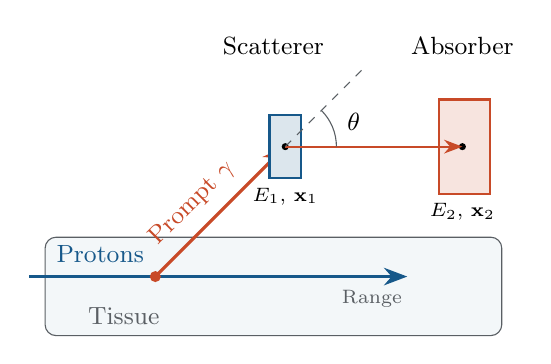
\begin{tikzpicture}[font=\small, >=Stealth]
        \filldraw[fill=crBlue!5,draw=crGrey,rounded corners]
          (0,0) rectangle (5.8,1.25);
        \node[crGrey] at (1.0,0.25) {Tissue};
        \draw[->,very thick,crBlue] (-0.2,0.75) -- (4.6,0.75);
        \node[above,crBlue] at (0.7,0.8) {Protons};
        \node[below,crGrey,font=\scriptsize] at (4.15,0.7) {Range};
        \fill[crRed] (1.4,0.75) circle (0.07);
        \draw[->,very thick,crRed] (1.4,0.75) -- (3.05,2.4);
        \node[rotate=45,above,crRed] at (2.05,1.5) {Prompt $\gamma$};
        \filldraw[fill=crBlue!15,draw=crBlue,thick]
          (2.85,2.0) rectangle (3.25,2.8);
        \filldraw[fill=crRed!15,draw=crRed,thick]
          (5.0,1.8) rectangle (5.65,3.0);
        \fill (3.05,2.4) circle (0.045);
        \fill (5.3,2.4) circle (0.045);
        \draw[->,thick,crRed] (3.05,2.4) -- (5.3,2.4);
        \draw[dashed,crGrey] (3.05,2.4) -- (4.05,3.4);
        \draw[crGrey] (3.7,2.4) arc[start angle=0,end angle=45,radius=0.65];
        \node at (3.92,2.72) {$\theta$};
        \node[above,align=center] at (2.9,3.45) {Scatterer};
        \node[above,align=center] at (5.3,3.45) {Absorber};
        \node[below,font=\scriptsize] at (3.05,2.0) {$E_1,\,\mathbf{x}_1$};
        \node[below,font=\scriptsize] at (5.3,1.8) {$E_2,\,\mathbf{x}_2$};
      \end{tikzpicture}}\\[2mm]
      {\scriptsize\color{crGrey} One photon, two detector interactions:
       Compton scattering followed by absorption.}\\[3mm]
      {\tiny\color{crGrey}
       \href{https://doi.org/10.3389/fonc.2016.00080}
       {Hueso-Gonz\'alez et al., Front. Oncol. 6:80 (2016).}\\
       \href{https://arxiv.org/abs/2202.06556}
       {Hybrid in-beam PET and Compton imaging (2022).}}
    \end{column}
  \end{columns}
\end{frame}

\begin{frame}{PET in proton therapy in brain}
  \begin{columns}[T]
    \begin{column}{0.58\textwidth}
      \begin{itemize}
        \item \hi{Rigid, reproducible positioning} --- the target sits in the
          same place every fraction.
        \item Compact, well-defined anatomy: a \hi{short field of view} covers
          it comfortably.
        \item High clinical stakes: paediatric and skull-base tumours next to
          critical structures.
        \item Our illustrative case: a \hi{fourth-ventricle ependymoma}.
      \end{itemize}
    \end{column}
    \begin{column}{0.42\textwidth}
      \centering
      
\includegraphics[height=0.42\textheight]{ependymoma_mri.png}\\
      {\scriptsize\color{crGrey} Fourth-ventricle ependymoma (MRI).}
    \end{column}
  \end{columns}
\end{frame}

\begin{frame}{Head phantom used in the simulation}
  \centering
  
\includegraphics[height=0.82\textheight]{mird_head.png}
\end{frame}

% ===========================================================================
\section{State of the art}

\begin{frame}{PET range verification: offline, in-beam and in-room}
  \centering
  
\includegraphics[width=0.94\textwidth,height=0.80\textheight,keepaspectratio]{in-room.png}
\end{frame}

\begin{frame}{PET range verification: offline, in-beam and in-room}
  \centering
  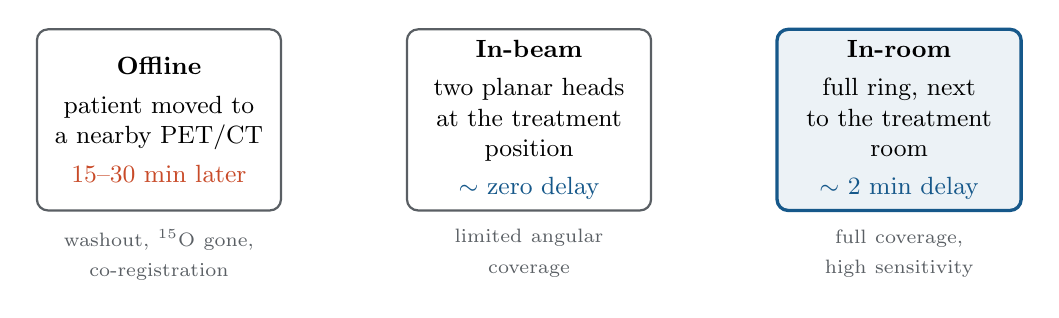
\begin{tikzpicture}[font=\small, node distance=6mm]
    % offline
    \node[draw=crGrey, rounded corners, minimum width=3.1cm, minimum height=2.3cm,
          align=center, thick] (off) at (0,0)
      {\textbf{Offline}\\[1mm] patient moved to\\ a nearby PET/CT\\[1mm]
       \textcolor{crRed}{15--30 min later}};
    % in-beam
    \node[draw=crGrey, rounded corners, minimum width=3.1cm, minimum height=2.3cm,
          align=center, thick] (ib) at (4.7,0)
      {\textbf{In-beam}\\[1mm] two planar heads\\ at the treatment\\ position\\[1mm]
       \textcolor{crBlue}{$\sim$ zero delay}};
    % in-room
    \node[draw=crBlue, fill=crBlue!8, rounded corners, minimum width=3.1cm,
          minimum height=2.3cm, align=center, very thick] (ir) at (9.4,0)
      {\textbf{In-room}\\[1mm] full ring, next\\ to the treatment\\ room\\[1mm]
       \textcolor{crBlue}{$\sim$ 2 min delay}};
    \node[below=1mm of off, text width=3.1cm, align=center, crGrey]
      {\scriptsize washout, \OT\ gone,\\ co-registration};
    \node[below=1mm of ib, text width=3.1cm, align=center, crGrey]
      {\scriptsize limited angular\\ coverage};
    \node[below=1mm of ir, text width=3.1cm, align=center, crGrey]
      {\scriptsize full coverage,\\ high sensitivity};
  \end{tikzpicture}
  \vspace{2mm}

  {\color{crGrey}\small The trade-off is \textbf{delay} vs.\ \textbf{angular
   coverage / scanner quality}.}
\end{frame}

\begin{frame}{Offline results in large uncertainties}
  \begin{columns}[T]
    \begin{column}{0.56\textwidth}
      A delay of 15--30 minutes costs on three fronts:
      \begin{itemize}
        \item \hi{Sensitivity}: the abundant \OT\ (2\,min) has vanished --- only
          the sparse \CE\ tail remains.
        \item \hi{Biological washout}: perfusion clears the emitters; hard to
          model, patient-dependent.
        \item \hi{Co-registration}: the patient is set up afresh on a separate
          scanner --- a few-mm misalignment maps straight into an apparent
          range shift.
      \end{itemize}
      \vspace{1mm}
%      {\small\color{crGrey} Literature: offline accuracy a few mm at best
%       (Knopf 2009; Parodi).}
    \end{column}
    \begin{column}{0.44\textwidth}
      \centering
      
\includegraphics[width=\linewidth]{activity.png}\\
      {\scriptsize\color{crGrey} \OT\ dominates the first minutes, then decays;
       \CE\ carries the late, weak signal.}
    \end{column}
  \end{columns}
\end{frame}

\begin{frame}{Online/In-room tradeoffs}
  \begin{columns}[T]
    \begin{column}{0.5\textwidth}
      \textbf{\color{crBlue}In-beam} (short delay, same bed)
      \begin{itemize}
        \item Retains the short-lived \OT, essentially no delay.
        \item But the beam must pass: only \hi{two planar heads} fit.
        \item Reduced angular coverage $\Rightarrow$ \hi{low sensitivity} and
          limited-angle image artefacts.
      \end{itemize}
    \end{column}
    \begin{column}{0.5\textwidth}
      \textbf{\color{crBlue}In-room} (just after, full ring)
      \begin{itemize}
        \item A \hi{full closed ring} $\Rightarrow$ full coverage, high
          sensitivity, clean image.
        \item Same couch $\Rightarrow$ a known rigid transform and a short
          transfer, without separate-scanner repositioning.
        \item The $\sim$2-min delay is \hi{bought back} by sensitivity and a
          \hi{better scanner}.
      \end{itemize}
    \end{column}
  \end{columns}
  \vspace{2mm}
  \begin{center}
    \fbox{\parbox{0.9\textwidth}{\centering
      A \hi{high-sensitivity in-room ring} combines short transfer time with
      complete angular coverage and high sensitivity.}}
  \end{center}
\end{frame}

% ===========================================================================
\section{CRYSP}

\begin{frame}{CRYSP: \emph{CRYogenic Sensitive PET}}
  \begin{columns}[T]
    \begin{column}{0.6\textwidth}
      \begin{itemize}
        \item Scintillators \hi{CsI and BGO} gain dramatically in light yield
          when cooled --- at 77 K, CsI reaches $\sim$100 photons/keV and BGO
          $\sim$29 photons/keV.
            \item In both cases, high yields translate into excellent energy resolution
              (6\% CsI, 10\% BGO),
              which in turn is essential for efficient scatter rejection.
        \item Monolithic crystals + SiPMs permit 3D position reconstruction using neural
              networks with high accuracy and no parallax error.
      \end{itemize}

    \end{column}
    \begin{column}{0.4\textwidth}
      \centering
      
\includegraphics[width=1.08\linewidth]{3D.png}\\
      {\scriptsize\color{crGrey} 3D reconstruction in a monolithic crystal.}
    \end{column}
  \end{columns}
\end{frame}

%\begin{frame}{One concept, a family of scanners}
%  \centering
%  \begin{tabular}{lccc}
%    \toprule
%    Configuration & Axial FOV & Inner radius & Role \\
%    \midrule
%    \textbf{TBP} (reference)   & 1024\,mm & 387\,mm & total-body reach \\
%    \textbf{LAFOV}             & 512\,mm  & 350\,mm & most indications \\
%    \textbf{CAFOV}             & 358\,mm  & 350\,mm & head / skull-base \\
%    \bottomrule
%  \end{tabular}
%  \vspace{3mm}
%  \begin{itemize}
%    \item Monolithic CsI or BGO, $48\times48$\,mm$^2$, 2 radiation lengths deep.
%    \item Head and skull-base targets fit the \hi{compact} configuration ---
%      cheaper, and enough.
%    \item Longer axes buy sensitivity and reach for craniospinal / body sites.
%  \end{itemize}
%\end{frame}

\begin{frame}{Scanner cost breakdown}
  \centering
  
\includegraphics[width=0.94\textwidth,height=0.80\textheight,keepaspectratio]{cost_breakdown.png}
\end{frame}

\begin{frame}{Total scanner cost}
  \centering
  
\includegraphics[width=0.94\textwidth,height=0.80\textheight,keepaspectratio]{scanner_totals.png}
\end{frame}

% ===========================================================================
\section{Results}

\begin{frame}{Imaging the brain}
  \centering
  
\includegraphics[width=0.88\textwidth,height=0.36\textheight,keepaspectratio]{recon_projections_bgo.png}\\[2mm]
  
\includegraphics[width=0.88\textwidth,height=0.36\textheight,keepaspectratio]{fit_all_events_bgo.png}
\end{frame}

\begin{frame}{Statistical procedure: from simulations to range precision}
  \begin{columns}[T]
    \begin{column}{0.44\textwidth}
      \begin{itemize}
        \item Ten independent 1\,Gy simulations provide the parent event pool.
        \item $N=100$ independently thinned realisations estimate the
          run-to-run spread of the fitted activity midpoint, $R_{50}$.
        \item A finite-pool correction restores the count variance of independent
          acquisitions.
        \item Reference BGO: \hi{0.070\,mm nominal} and
          \hi{0.101\,mm with washout}.
      \end{itemize}
    \end{column}
    \begin{column}{0.56\textwidth}
      \centering
      
\includegraphics[width=\linewidth]{statistical_procedure_bgo.png}\\
      {\scriptsize\color{crGrey} Reference TBP BGO study: one shard and the
       washed $N=100$ ensemble.}
    \end{column}
  \end{columns}
\end{frame}

\begin{frame}{Reference protocol: all scanner configurations are sub-mm}
  \begin{columns}[T]
    \begin{column}{0.44\textwidth}
      \begin{itemize}
        \item \hi{Protocol:} 1\,Gy, 300\,s acquisition, starting 120\,s after
          beam-off; washout included.
        \item BGO: \hi{0.101--0.127\,mm}; CsI: \hi{0.146--0.155\,mm}.
        \item BGO is more precise through higher sensitivity; CsI remains a
          competitive, lower-cost option.
        \item These values are the \hi{statistical precision of the fitted
          activity edge}.
      \end{itemize}
    \end{column}
    \begin{column}{0.56\textwidth}
      \centering
      
\includegraphics[width=\linewidth]{statproc_washed_grid.png}\\
      {\scriptsize\color{crGrey} Finite-pool-corrected $\sigma_R$ for the
       reference protocol ($N=100$).}
    \end{column}
  \end{columns}
\end{frame}

\begin{frame}{Timing flexibility: the CsI stress case remains below 0.35 mm}
  \begin{columns}[T]
    \begin{column}{0.44\textwidth}
      \begin{itemize}
        \item CsI is the lower-cost, less precise crystal; BGO is more precise
          at every configuration studied.
        \item At a 300\,s start delay, $\sigma_R$ is 0.266\,mm for a 300\,s
          scan and 0.324\,mm for a 120\,s scan.
        \item Across all tested delays and scan durations,
          \hi{$\sigma_R<0.35$\,mm}.
        \item The scanner contribution is therefore well below the
          1\,mm target.
      \end{itemize}
    \end{column}
    \begin{column}{0.56\textwidth}
      \centering
      
\includegraphics[width=\linewidth]{statproc_delay_csi.png}\\
      {\scriptsize\color{crGrey} CsI range precision vs.\ start delay, with
       washout ($N=100$).}
    \end{column}
  \end{columns}
\end{frame}

% ===========================================================================
\section{Summary}

\begin{frame}{Summary}
  \begin{itemize}
    \item Proton-therapy range verification needs an \hi{in vivo}, online/in-room,
      high-sensitivity probe
    \item \hi{CRYSP in-room PET} exploits cryogenic CsI/BGO for excellent energy
      and spatial resolution at a \hi{competitive cost}.
    \item For the reference protocol, the fitted activity edge has
      \hi{0.101--0.155\,mm statistical precision} across all BGO and CsI
      geometries; the tested CsI timing grid remains below 0.35\,mm.
    \item CsI offers a very good, low-cost, supply-secure option; BGO offers
      the best statistical precision.
  \end{itemize}
  \vspace{3mm}
\end{frame}

{\setbeamertemplate{footline}{}
\begin{frame}[plain]
  \centering
  {\color{crBlue}\Large Thank you}\\[3mm]
  {\color{crGrey} Questions --- and collaborations --- welcome.}
\end{frame}}

\end{document}
